\documentclass[druk]{dyplom}
\usepackage[utf8]{inputenc}
\usepackage{hyperref}
%%
\usepackage[toc]{appendix}
\renewcommand{\appendixtocname}{Dodatki}
\renewcommand{\appendixpagename}{Dodatki}
\usepackage[english]{babel}
%usepackage{titlesec}

% pakiet do składu listingów w razie potrzeby można odblokować możliwość numerowania linii lub zmienić wielkość czcionki w listingu
\usepackage{minted}
\setminted{breaklines,
frame=lines,
framesep=5mm,
baselinestretch=1.1,
fontsize=\small,
%linenos
}

% nowe otoczenie do składania listingów
\usepackage{float}
\newfloat{listing}{htp}{lop}
\floatname{listing}{Listing}
\usepackage{chngcntr}
\counterwithin{listing}{chapter}

% patch wyrównujący spis listingów do lewego marginesu 
%https://tex.stackexchange.com/questions/58469/why-are-listof-and-listoffigures-styled-differently
\makeatletter
\renewcommand*{\listof}[2]{%
  \@ifundefined{ext@#1}{\float@error{#1}}{%
    \expandafter\let\csname l@#1\endcsname \l@figure  % <- use layout of figure
    \float@listhead{#2}%
    \begingroup
      \setlength\parskip{0pt plus 1pt}%               % <- or drop this line completely
      \@starttoc{\@nameuse{ext@#1}}%
    \endgroup}}
\makeatother

\usepackage{url}
\usepackage{lipsum}

% Dane o pracy
\author{Yuriy Slinkin}
\title{Evolutionary methods efficiency optimization using distributed systems}
\promotor{dr inż. Michał Przewoźniczek}
%\konsultant{dr hab. inż. Kazimerz Kabacki}
\wydzial{Faculty of Computer Science and Management}
\kierunek{Computer Science}
\krotkiestreszczenie{This thesis presents an optimization of genetic algorithms using parallelization and distributed computing, bounded in programming library.}
\slowakluczowe{evolutionary methods, genetic algorithm, optimization, distributed computing, parallelization}

\begin{document}

%\maketitle

\tableofcontents

\listoffigures

\listof{listing}{List of Listings}

\listoftables

%\pagebreak

% --- Strona ze streszczeniem i abstraktem ------------------------------------------------------------------

\chapter{Abstract}

Nowadays artificial intelligence (AI) is gaining its popularity and changing more and more domains with its growth. Algorithms and heuristics are capable of some non-trivial things, that until the recent time was known to be impossible for a machine. In some particular cases, artificial intelligence methods perform tasks a lot better than a human being. However, there are still a lot of uncovered domains, where AI is not yet as good as it could be.

Evolutionary algorithms are one of the families of metaheuristic optimization algorithms. It is a subset of evolutionary computation, which was inspired by biological evolution. Its goal is to find the best solution for the given fitness function, which may be non-trivial and take over a lifetime to reach the same result by checking each possible solution.

The thesis addresses inconveniences regarding evolutionary algorithms and purposes solution introducing the concepts of parallelism and distributed computing. It notes the importance of evolutionary algorithms, and genetic algorithms in specific, and how it may be interesting for both scholars and professional developers. 

% Kilka sztuczek, żeby:
% - Abstract pojawił się na tej samej stronie co Streszczenie
% - Abstract nie pojawił się w spisie treści
\iffalse
\addtocontents{toc}{\protect\setcounter{tocdepth}{-1}}
\begingroup
\endgroup
\addtocontents{toc}{\protect\setcounter{tocdepth}{2}}
% --- Koniec strony ze streszczeniem i abstraktem 
\renewcommand{\cleardoublepage}{}
\renewcommand{\clearpage}{}
\fi

\chapter*{Goals}

This theses is driven by the need for improvements among evolutionary computation domain. The theses has two objectives.

The first aim of the thesis is to analyze how parallelization and distributed computing may be applied to optimize evolutionary algorithms workflow. By its nature it should increase performance of such methods and allow horizontal scaling.

The second goal of the thesis is to gather common logic of genetic algorithms, containing the improvements done introduced by previous analysis, into powerful and convenient tool for creating and integration of genetic algorithms with different applications for solving theoretical and practical problems of all levels of complexity.

\chapter*{Outline}

This thesis addresses the main weaknesses of evolutionary methods using the example of genetic algorithms, the most frequently encountered type of evolutionary algorithm. This is inflexibility and time consumption. First, genetic algorithms are usually designed for specific problem, making it insufficient for reusage, so new implementation of the algorithm needs the same amount of work. Second, genetic algorithms are used to solve complex, multi-dimensional problems, which may take up to days or even months to find a solution. Optimization of such algorithms is very beneficial, as even the small relative performance increase may safe days of computations. An abstract solution with its functional and non-functional requirements was proposed, constructing the idea of how these addressed problems could be resolved. The existing solutions were taken under consideration, describing their advantages and disadvantages. Then author's application was described, how it was built and how it meets all predefined requirements. Finally the set of experiments was performed in order to observe the performance increase achieved with the usage of proposed solution solving one of the combinatorial optimization problems.


-----------------------------------------------------------
\renewcommand{\labelitemi}{$\bullet$}
\renewcommand{\labelitemii}{$\cdot$}
\renewcommand{\labelitemiii}{$\diamond$}
\renewcommand{\labelitemiv}{$\ast$}


\chapter{Background}

\section{Domain overview}

In artificial intelligence, an evolutionary algorithm (EA) is a subset of evolutionary computation, a generic population-based metaheuristic optimization algorithm. An EA uses mechanisms inspired by biological evolution, such as reproduction, mutation, recombination, and selection. Candidate solutions to the optimization problem play the role of individuals in a population, and the fitness function determines the quality of the solutions. Evolution of the population then takes place after the repeated application of the above operators.

Evolutionary algorithms often perform well approximating solutions to all types of problems because they ideally do not make any assumption about the underlying fitness landscape. Techniques from evolutionary algorithms applied to the modeling of biological evolution are generally limited to explorations of microevolutionary processes and planning models based upon cellular processes. In most real applications of EAs, computational complexity is a prohibiting factor. In fact, this computational complexity is due to fitness function evaluation. Fitness approximation is one of the solutions to overcome this difficulty. However, seemingly simple EA can solve often complex problems[citation needed]; therefore, there may be no direct link between algorithm complexity and problem complexity.

Overall the optimization methods can be divided generally into two groups: the gradient methods, that operate on a single potential solution and look for some improvements in its neighborhood, and global optimization techniques – represented here by so called evolutionary methods – that maintain large sets (populations) of potential solutions and apply some recombination and selection operators on them. During the last decades, evolutionary methods have received a considerable attraction and have experienced a rapid development. Main paradigms are: genetic algorithm (binary or real coded), augmented simulated annealing (binary or real coded), evolution strategy and differential evolution. Still, each of these methods has many possible improvements.
In this theses the author is concentrating on subfamily of evolution methods named genetic algorithms. It is one of the most popular representative of evolutionary methods and serves as a great example, because it allows to observe and study the properties of the whole family.

\subsection{How evolutionary algorithms are used nowadays?}

Typically, optimization methods arising in engineering design problems are computationally demanding because they require evaluation of a quite complicated objective function many times for different potential solutions. Moreover, the objective function is often multi-modal, non-smooth or even discontinuous, which means that traditional, gradient-based optimization algorithms fail and global optimization techniques, which generally need even a larger number of function calls, must be employed. Fortunately, the rapid development of computational technologies and hardware components allows us to treat these problems within a reasonable time.

Genetic algorithms have been applied in science, engineering, business and social sciences. Number of scientists has already solved many engineering problems using genetic algorithms. GA concepts can be applied to the engineering problem such as optimization of gas pipeline systems. Another important current area is structure optimization. The main objective in this problem is to minimize the weight of the structure subjected to maximum and minimum stress constrains on each member. GA is also used in medical imaging system. The GA is used to perform image registration as a part of larger digital subtraction angiographies. It can be found that GAs can be used over a wide range of applications \cite{introduction_to_ga}. Genetic algorithms can also be applied to production planning, air traffic problems, automobile, signal processing, communication networks, environmental engineering and so on. There is a lot of examples discussed in \cite{creative_ga} from music, art in general, architecture and engineering design.

\subsection{Disadvantages}
As every other technique, genetic algorithm has its flaws. In this theses the author tries to attract attantion to the two most important disadvantage of genetic algorithms, due to subjective opinion. For each of them is proposed an alternative solution, which will later take place in functional requirements of the thesis work.

\begin{enumerate}
\item \textbf{Implementation complexity}

There are many problems of different types, which may me optimized by genetic algorithms. The downside is that for each of those problems there is a need of specific implementation, which is at least time consuming. Even though the low level details, which depend on the problem GA is applied to, will change, the high level abstraction of genetic algorithm workflow remains the same: a population of individuals are processed in pipeline of genetic operators, resulting in a new fitter population.

A solution for this problem would be a high level generic representation of genetic algorithm, which may be reusable among variety of application and independent from the low level details. 
\medbreak

\item \textbf{Computation cost}

Genetic algorithms tend to be very time consuming. This is strictly related to its computation model, as the function, used in GA, are usually very demanding.

This characteristic of genetic algorithms, however, may be negated by the usage of parallelization.
\medbreak

\end{enumerate}

\section{Solution proposal}

A solution for described flaws would be a tool, which allows to integrate a high-performance implementation of the genetic algorithm into user application and use it for the arbitrary optimization problem with minimum changes required to the existing codebase. Additionally, this should be a convenient toolbox for theoretical and practical problems which might be resolved using genetic algorithms, providing a ready-made implementation of the most popular algorithms with extra features, which save users from implementing one themselves. For a solution to be considered as fulfilled, it is neccessary to meet both functional and non-functional requirements predifined in advance.

\subsection{Non-functional requirements}
\begin{enumerate}
\item \textbf{Java Virtual Machine}

This platform was chosen, because of its popularity and open nature. Java virtual machine is supported by many languages, what allows a user to pick a specific one, which is the best for a given circumstances. JVM is also vastly used and run on over 3 billion devices\footnote{According to official information provided by Oracle Corporation}.
\medbreak

\item \textbf{Open implementation}

The implementation of the tool has to be open to its users, allowing to view and expand source code to the specific needs. 
\medbreak

\item \label{nfreq:modul}\textbf{Modular architecture}

The architecture solution used to build the tool has contain modularity among its fundamentals. This means, that allowing different features, its components have to be grouped according to their functions, so the users, who are interested in a small part of provided functionality wouldn't be forced to use all capabilities of the tool.

\end{enumerate}

\subsection{Functional requirements}
\begin{enumerate}
\item \label{freq:stop} \textbf{Limiting the evolution in terms of time and/or number of iterations}
This is basic requirement for every genetic algorithm implementation. Evolution process takes time and in order to benefit from it, user must have access to the evolved version of population. Number of iterations corresponds to the number of evolution cycles performed on the population, when every genetic operator is applyed to it. On the other hand, the actual time of the evolution may be changed even in terms of the same number of iterations, as it strongly depends on performance of genetic operators and fitness function, so in some cases time may be the only valid criterion, which decides that evolution process should be stopped. 
\medbreak

\item \label{freq:best} \textbf{Controll of the best individual through evolution}

During the evolution process, due to the chosen selection, crossover or mutation strategies, even the fittest individual may not end in the next population. As for business needs it is important to get the best solution ever discovered by algorithm, it is important to store reference to that candidate separately.
\medbreak

\item \label{freq:cache} \textbf{Fitness values caching}
In genetic algorithms, the computation of the fitenss function provides the largest computational load for the algorithm. Each population genration is composed of individuals who are formed from previous gneeration via cloning, crossover, or mutation. It is also common for the individual to migrate to the next population without a change or, less common, a crossover of two different individuals may produce a genotype that already has been discovered earlier. If this occurres rather frequently, it is unprofitable to compute the fitness value all over again. As a solution one may consider caching the results of fitness computation for later reusage. Although it noticeably increases the speed of algorithm, the cache tends to grow dramatically, so the coise of data structure for this purposes is extrimely important. 
\medbreak

\item \label{freq:par} \textbf{Parallel evolution processing}

Genetic algorithms are generally known as a time-consuming technique, as it is often used with complex, high-dimensional problems. Evolution cycle may take up to hours and days of continuous computing, depending on the parameters of the algorithm and hardware in use, which comes with a great cost and very low flexibility, as with every mistake or change was done to algorithm implementation, evolution needs to be re-executed. On the other hand, even small upgrades in speed may result as a major cost cut.

For this reason, it is highly important to use the maximum of the given resources, avoiding unreasonable workloads. It may be achieved through the computation parallelization between multiple virtual CPU cores within a single machine
\medbreak

\item \label{freq:async} \textbf{Asynchronous evaluation of fitness value}

The solution must allow to compute fitness values on different machine or even cluster of machines, as well as using different low-level programming language or some specific optimization, with no need to switch the entire application to another platform. This type of environment also fits perfectly to cloud computing solutions, as fitness evaluation is entirely isolated from the rest of application.
\medbreak

\item \label{freq:generic} \textbf{Generic representation of individual}

There is a wide set of problems which might be resolved using genetic algorithms. Still, this optimization technique is rarely used in business applications and mainly considered as a theoretical solution. One of the reasons for such phenomenon is the difficulty which comes with a try to use genetic algorithm optimization without a previous plan to do so. The process of reshaping the existing codebase in such way, so typical genetic algorithm could be applying often demands big costs and high level of understanding GA workflow and its possibilities.

Depending on the problem a user is trying to solve, a standard representation of each candidate solution would be an array of bits, integers or real numbers. The main property that makes these genetic representations convenient is that their parts are easily aligned due to their fixed size, which facilitates simple crossover operations. For the purposes of genetic programming and evolutionary programming tree-like and graph-form representation are used respectively, which causes the necessity in different implementations for each problem.

A solution to this problem is an implementation of the genetic algorithm, which is able to work on generic types, which represents a candidate solution for the applied problem. Due to this property, it is possible to reuse the implementation for different problems and create a generic tool, which is decoupled from the problem it is applied to.
\medbreak

\item \label{freq:distributed} \textbf{Evolution in distributed environment}

As already mentioned, parallelization is a big part of speed optimization for genetic algorithms. While local parallelization is usefull and convinient for medium- and small-sized problems, working with complex use cases often demands the resources, which is may not fit into one machine. Distributed environment is a next step of parallelization, when evolution process is split between different machines, each computing its own part of the workload. This approach enables horizontal scaling, when each added machine increases performance of the algorithm.  
\medbreak

\item \label{freq:on-demand} \textbf{On-demand evolution}

Genetic algorithm optimization is generally used for finding the best solution for a defined problem, which is the fittest candidate to the provided fitness function. It means, that the best solution is defined relative to all the solutions assigned earlier and cannot be proved as the optimal one, even when it is. But when applying to a nontrivial problem, finding the optimal solution is not always cost-effective, as it may take up to exponential time. For this reason, it is common to compute a 'good enough' solution in reasonable time. Depending on the business reasons, this time varies so sometimes it is possible to wait until the better solution is computed and sometimes it is not. For instance, if the application which uses genetic algorithm has a real-time interface and its user is interested in gaining a solution for the particular case in the range of seconds, it is justifiable to provide a solution which may not be optimal but is close to it.

On the other hand, when a user is ready to allow the application to take its time in order to provide a better result, it has to still be possible to resume the evolution. Again the application should not limit users in such important cases, as the end user needs may vary depending on different circumstances, which may not be predicted in advance. The evolution of a solution to a given problem should be available on-demand, without forcing unreasonable resource uses, and adjust to a specific case as much as possible.
\medbreak
\end{enumerate}

\chapter{Existing solutions overview}

\section{Java Jenetics}

\section{Apache.math.genetics}

\chapter{Author's solution}

This chapter contains a description of the application created within the thesis, which is proposed as a concrete solution for previously addressed problems. The application is described from implementation perspective, its applicability for the end user and how it meets the predefined requirements.

\section{Implementation overview}

The solution is presented as an open-source library, that provides the major part of genetic algorithm implementation, which can be shared between different application. Base algorithm consist of a pipeline separated by three stages: selection, crossover and mutation, which evolves the population of individuals, increasing average level of adjustment and finding the best individual according to provided fitness function; preimplemented most popular strategies of genetic selection, crossover and mutation, with possibility of extanding with the additional ones for specific reasons and a set of platforms which allow to run the pipeline in a different ways, best suited for existing hardware. The library is supplied with key features, basing on the concepts described earlier, wrapping all the components into sufficient framework.

\subsection{Technology stack}

\subsubsection{Scala programming language}

Scala is a modern multi-paradigm programming language designed to express common programming patterns in a concise, elegant, and type-safe way. Its name stands for "scalable language." The language is so named because it was designed to grow with the demands of its users. It can be applied to a wide range of programming tasks, from writing small scripts to building large systems.
Scala is easy to get into. It runs on the standard Java platform and interoperates seamlessly with all Java libraries. It's quite a good language for writing scripts that pull together Java components. But it can apply its strengths even more when used for building large systems and frameworks of reusable components. \cite{programming_in_scala}

Technically, Scala is a blend of object-oriented and functional programming concepts in a statically typed language. The fusion of object-oriented and functional programming shows up in many different aspects of Scala; it is probably more pervasive than in any other widely used language. The two programming styles have complementary strengths when it comes to scalability. Scala's functional programming constructs make it easy to build interesting things quickly from simple parts. Its object-oriented constructs make it easy to structure larger systems and adapt them to new demands. The combination of both styles in ScaalMatei Zaharia, “Spark: Cluster Computing with Working Sets
 makes it possible to express new kinds of programming patterns and component abstractions. It also leads to a legible and concise programming style \cite{programming_in_scala}

% May be expanded with definitions from books

Due to its programming style and variety of features Scala serves a great tool for developing this library. A combination of paradigms is extremely usefull in this case and was crutial during selection of programming language. Both of the programming styles were heavily used in order to gain the best possible result:
\begin{itemize}
\item
Object-oriented style

Scala is an object-oriented language in pure form: every value is an object and every operation is a method call. \cite{programming_in_scala} It provides modularity and maintainability: all application is split into a self-sufficient containers, which store the relevant data and provide available operations, that may be performed on its data. These containers may be used as the assembling parts for another container, passed as function parameter and returned as function result. Such approach allows to keep track of the growing codebase, alligning its components into domain hierarchies and letting its parts to comunicate with one another.

\item
Functional style

Functional programming provides expressiveness, composability and conciseness. Building the library with mathematical-like functions makes it more understandable, replacing the mutable state from the application. As the result, it becomes clear, unequivocal and may be safely used in multi-thread environment. One of the most important assets, which comes from functional programming, is scalability. A well constructed application may easily be enlarged for user needs to handle a growing amount of work; it is more adaptive to the changing needs and the performance of such system improves proportionally to the additional hardware.

\end{itemize} 

 \textbf{Parallel collections}

 Encouraging usage of immutable objects, from version 2.8 Scala provides new collection API, which contains parallel collections package as part of it. Parallel collections were included in the Scala standard library in an effort to facilitate parallel programming by sparing users from low-level parallelization details, meanwhile providing them with a familiar and simple high-level abstraction. The idea is simple– collections are a well-understood and frequently-used programming abstraction. And given their regularity, they’re able to be efficiently parallelized, transparently. By allowing a user to “swap out” sequential collections for ones that are operated on in parallel, Scala’s parallel collections take a large step forward in enabling parallelism to be easily brought into more code. \cite{scala_parallel_collections_overview}

 How parallel collections are built?
 What may be acquired with scala parallel collections?


\subsubsection{Apache Spark}

Apache Spark is a high-performance, general-purpose distributed computing system that has become the most active Apache open source project, with more than 1,000 active contributors. Spark enables users to process large quantities of data, beyond what can fit on a single machine, with a high-level, relatively easy-to-use API. Spark’s design and interface are unique, and it is one of the fastest systems of its kind. Uniquely, Spark allows to write the logic of data transformations and machine learning algorithms in a way that is parallelizable, but relatively system agnostic. So it is often possible to write computations that are fast for distributed storage systems of varying kind and size.

On the generality side, Spark is designed to cover a wide range of workloads that previously required separate distributed systems, including batch applications, iterative algorithms, interactive queries, and streaming. By supporting these workloads in the same engine, Spark makes it easy and inexpensive to combine different processing types, which is often necessary in production data analysis pipelines.\cite{learning_spark}

Spark can run over a variety of cluster managers to access the machines in a cluster. The easiest way is to run Spark by iteself on a set of machines. For this purpose Spark comes with built-in Standalone mode. Spark’s Standalone manager offers a simple way to run applications on a cluster. It consists of a master and multiple workers, each with a configured amount of memory and CPU cores. When application is submited, one can choose how much memory its executors will use, as well as the total number of cores across all executors.

Spark Core contains the basic functionality of Spark, including components for task scheduling, memory management, fault recovery, interacting with storage systems, and more. Spark Core is also home to the API that defines resilient distributed data‐sets (RDDs), which are Spark’s main programming abstraction. RDDs represent a collection of items distributed across many compute nodes that can be manipulated in parallel. Spark Core provides many APIs for building and manipulating these collections. RDDs offer two types of operations: transformations and actions. Transformations construct a new RDD from a previous one. For example, one common transformation is filtering data that matches a predicate. Actions are operations, which produce different result than the transformation, like collecting the elements into a local collection on master node or counting the number of elements in RDD. Transformations and actions are different because of the way Spark computes RDDs. Although new RDDs can be defined in any time, Spark computes them only in a lazy fashion — that is, the first time they are used in an action. The transformations, on the other hand, are scheduled to a DAG (directed acyclic graph) of computations. This approach has a lot of advantages, among them: effective fault tollerance and ability to make a lot of optimization decisions before actually running operations. This would not be possible if it executed computations as soon as it got it.

In distributed mode, Spark uses a master/slave architecture with one central coordinator and many distributed workers. The central coordinator is called the driver. The driver communicates with a potentially large number of distributed workers called executors. The driver runs in its own Java process and each executor is a separate Java process. A driver and its executors are together termed a Spark application. Then a Spark application is launched on a set of machines using early described cluster manager.

\begin{figure}
\centering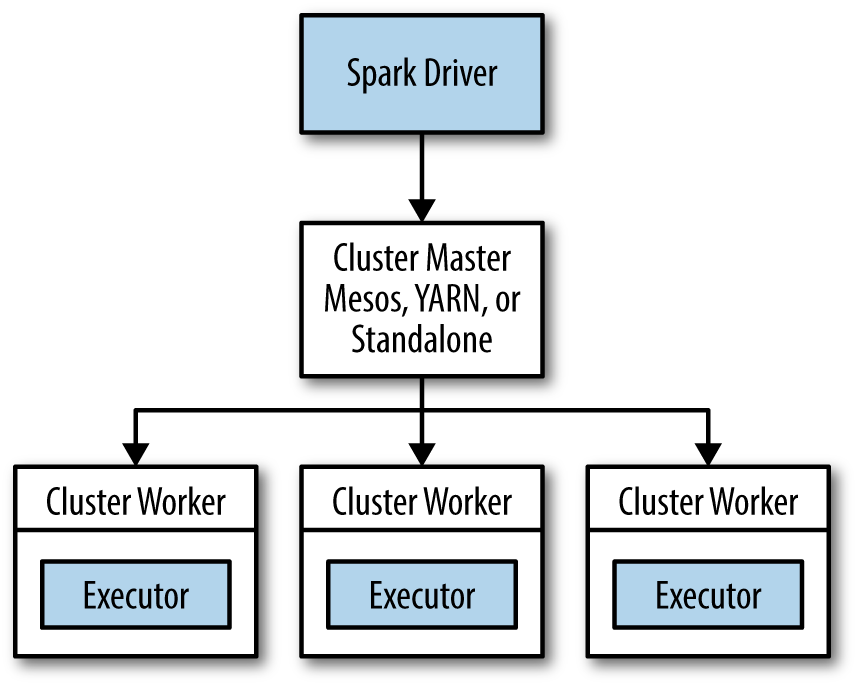
\includegraphics[width=.6\textwidth]{img/spark-runtime-split}
\caption{ The components of a distributed Spark application \cite{learning_spark}.}  \label{img:spark-components}
\end{figure}

This architectures allows to distribute the data between different executor nodes and perform operations on it locally until the shuffling is needed. Only then the data is shared between different nodes and the network communication is handled. In a distributed program, communication is very expensive, so laying out data to minimize network traffic can greatly improve performance. Much like how a single-node program needs to choose the right data structure for a collection of records, Spark programs can choose to control their RDDs’ partitioning to reduce communication.

In order to be able to transforms large sets of data without redundant recomputation Spark provides data persistence. When the Spark is asked to persist an RDD, the nodes that compute the RDD store their partitions. Spark has many levels of persistence to choose from based on what the goals are. The list of storage levels with performance comparison may is shown on \ref{img:spark_persistence_levels}. Combining different persistence modes, an executor can effectively share the data between its disk and RAM.

\begin{figure}
\centering 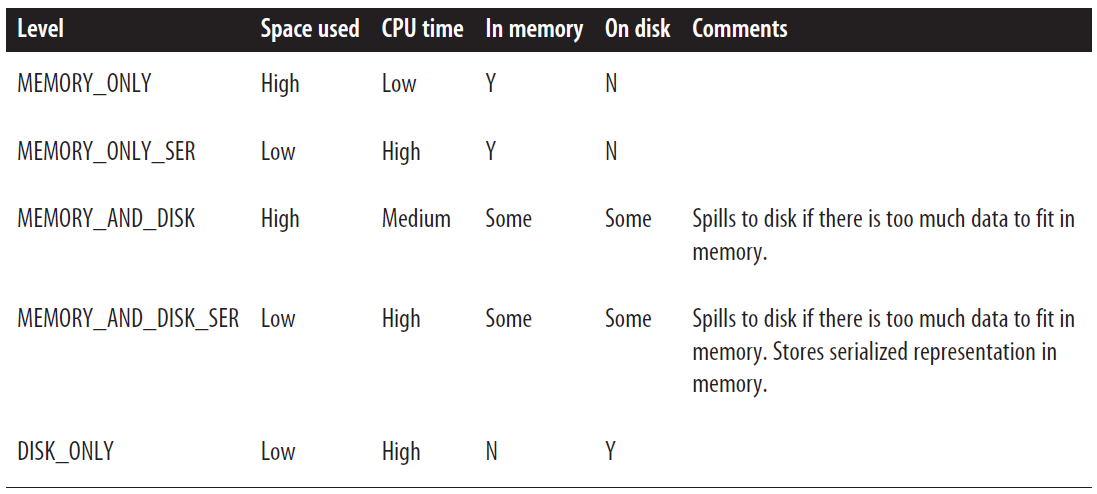
\includegraphics[width=.6\textwidth]{img/spark_persistence_levels}
\caption{ Persistence levels from org.apache.spark.storage.StorageLevel and
pyspark.StorageLevel \cite{learning_spark}.}\label{img:spark_persistence_levels}
\end{figure}



\subsubsection{Akka Streams}


Akka Streams is a library to process and transfer a sequence of elements using bounded buffer space. This latter property is what is ususally referred as boundedness and it is the defining feature of Akka Streams. Translated to everyday terms it is possible to express a chain of processing entities, each executing independently (and possibly concurrently) from the others while only buffering a limited number of elements at any given time. 

\begin{figure}
\centering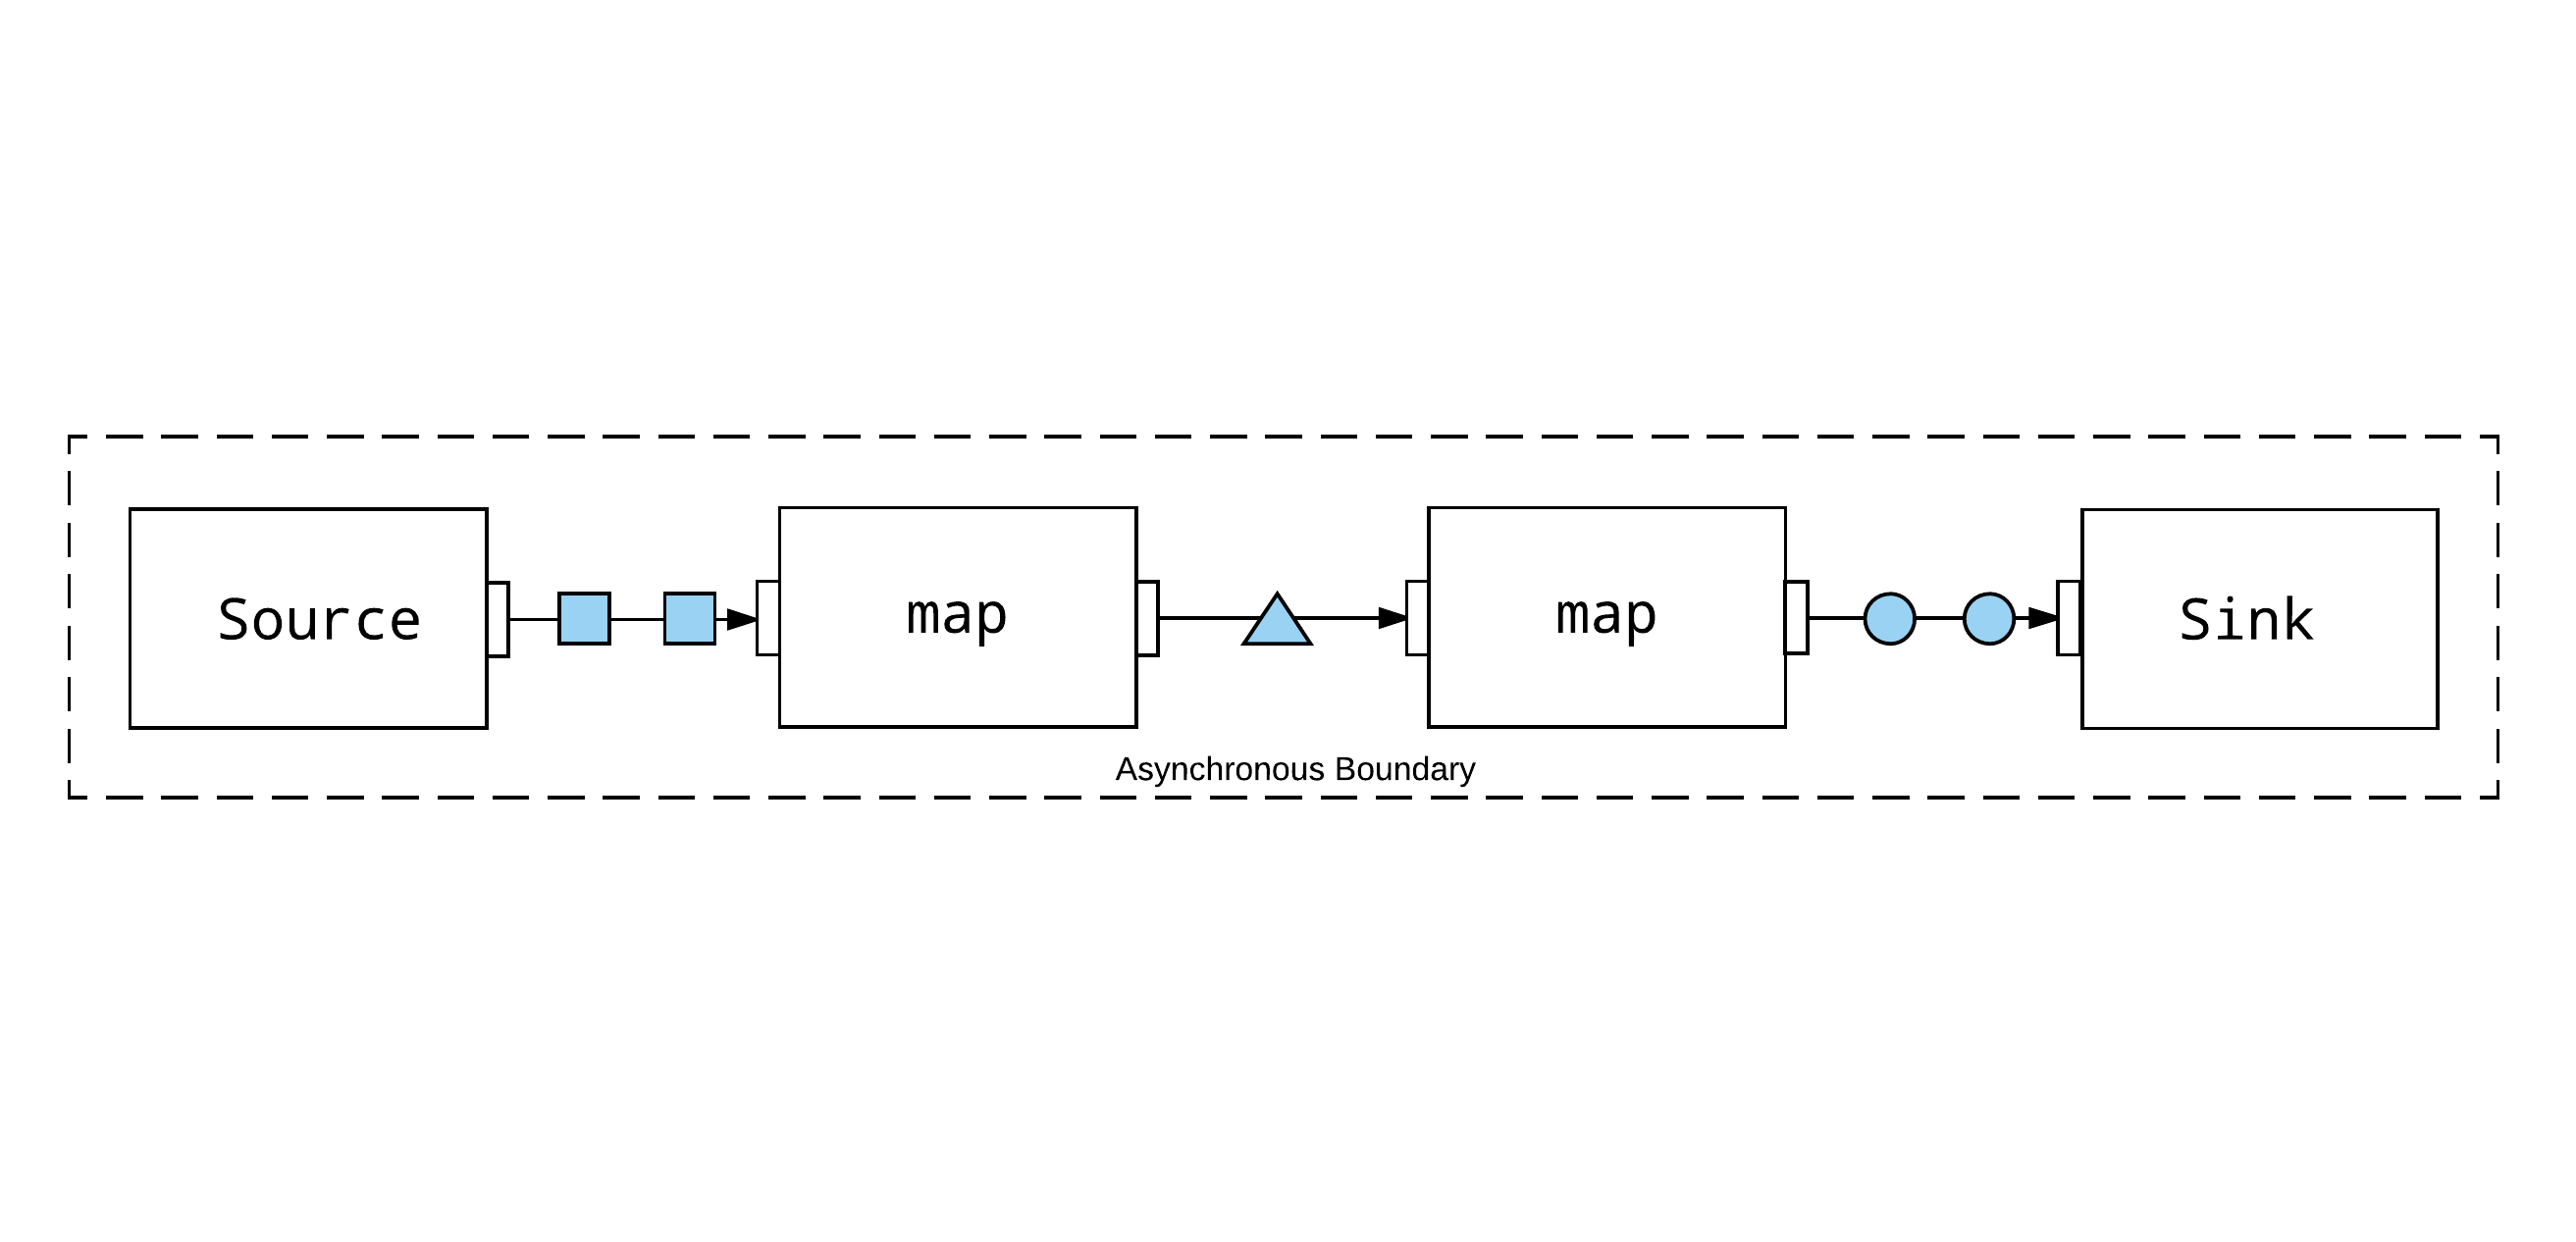
\includegraphics[width=.7\textwidth]{img/akka-streams-1}
\caption{A typical stream flow}\label{img:streams-1}
\end{figure}


\textit{ToDo: more info}


\subsection{Core components}

\textit{ToDo: add introduction}

\begin{itemize}

\item
Individual

An individual is a core component of genetic algorithm, often also reffered to as a \textit{genotype, chromosome \emph{or} a candidate}, which represents a candidate solution to a given problem. The number of individuals are evolved during the algorithm workflow, mixed and mutated in order to find the fittest one according to provided fitness function. This concept is purely abstract in the library, encoded as a generic type which may have an arbitrary representation defined by the users depending on their needs. 

In order to handle an individual through the process of evolution there should be defined a set of operators, where each encapsulates logic of some part of evolution procedure.   
\medbreak

\begin{itemize}
\item
Fitness

Fitness is a type class which represents a function of type \texttt{I => Double}, where \texttt{I} is type of individual. This function summarises how close a given design solution is to achieving the set aims. A ftness function must be devised for each problem to be solved, thus should be provided by the user and may not be preimplemented. Fitness function value is main criterion of future selection and is very important attribute of individual representation.

\textit{ToDo - how much does it cost}
\medbreak

\item
Join

Join is a type class, which represents a cross function of type \texttt{(I, I) => (I, I)}, where \texttt{I} is type of individual. This function defines how two instances of type \texttt{I} may be combined together to produce a new pair of \texttt{I}. It describes a crossover operation, due to which all the individuals from a population combined into pairs will be mixed during evolution process. An instance of the type class may be created from a single function of type \texttt{(I, I) => (I, I)}, as well as a function of type \texttt{(I, I) => I}. The latter case is suitable when identical function is used to compute both of result elements or in case of commutative operation. These cases were separated in order to enable memory allocation optimization by reusing the same product object to construct result pair.
\medbreak

\item
Modification

Modification is a type class, which represents a mutation function of type \texttt{I => I}, where \texttt{I} is type of individual. This operator is used to maintain generic diversity from one generation of a population to another. It is analogous to biological mutation. Mutation alters one or more gene values in a chromosome from its initial state, during which the solution may change entirely from the former shape. Because of its loose representation (even identity function may be considered as modification) it is important to provide a set of laws, which will distinguish a modification, which actually brings a diversity into the population. A \textit{lawfull} modification function is one, which holds following properties:

\begin{enumerate}
\item
A modified instance does not equal to original one (\textit{e.i modification function does not equal to identity function}) \ref{listing:mod1}

\begin{listing}
\begin{minted}{python}
	modify(i) != i
\end{minted}
\caption{The first laws of Modification instance} \label{listing:mod1}
\end{listing}

\item
After a certain number of modification the same input produces different outputs (\textit{ e.i. modification function is randomized or depends on outer variables}) \ref{listing:mod2}

\begin{listing}
\begin{minted}{python}
	def modify5(i: I) = modify(modify(modify(modify(modify(i)))))
	modify5(i) != modify5(i)
\end{minted}
\caption{The second laws of Modification instance} \label{listing:mod2}
\end{listing}


\end{enumerate}
\medbreak

\item
Scheme

Scheme is a type class, which is responsible for a creation of new individual. This is additional function, which may be replaced by predefined initial population during the start of evolution process, but still offers more functionality and may be used when individuals are created randomly, from limitless iteratator, smaller collection, which should be cycled or even single instance of individual. This concept is implemented as a covariant class, so the scheme object of parent class may be replaced by the scheme object of child class. It allows to easily use this class with hierarchies, avoiding redundant code. 
\end{itemize} 

\smallskip \textit{Together this satisfies predefined functional requirement \ref{freq:generic}}

\medbreak

\item
Population

Population is a collecion of individuals, which holds them during single evolution step. Individuals are processed together and are viewed only as a part of population from the perspective of algorithm. During the evolution step the representation of population or holding type may be changed (e.g. after selection stage further processed population contains pair of individuals, which are meant to be mixed later).

From implementation perspective, population is a type alias to Scala vector collection. The choise of data structure was motivated by fast average performance and effectively constant random access time in particular.
\medbreak

\item
Evolution environment

Evolution environment is a component, which taking the set of options constructs endless evolution flow of given population and makes it ready to be run. It is a parent type to all implementations of different approaches in processing computations, which may be sequential or parallel, local or distributed. This concept is very important from the usage perspective as it devides the implementation of genetic algorithm from its usage, so the end user may even not be aware of the way how the evolution is performed. It is also the end point of all the dependent components, as there is no direct dependency to any of concrete implementation of evolution environment. This abstraction may be considered as high level representation of genetic algorithm itself. The list of concrete derivatives of this interace contains:
\begin{itemize}
\item[--]
Local environment

This type of environment presumes local evoluation of evolution flow. It is the richest environments in terms of possible configurations. The logic, behind the strategy of applying genetic operators and evaluating fitness values is decoupled from one another into instances of \texttt{EvolutionCompanion} and \texttt{FitnessEvaluator} classes respectively. For each of the strategies the are sequential and parallel versions, with additional fitness caching option for repetitive individuals within population. Any fitness evaluation strategy may combined with any possible technique of applying genetic operators, creating a number of possibilites ready for use.
\smallskip\textit{This satisfies predefined functional requirement \ref{freq:par}}
\medbreak

\item[--]
Asynchronous environment

Asynchronous environment delegates the function of fitness evaluation to another system, by sending non-blocking asynchronous calls for every element of the population. It may be extremely usefull for the problems with heavy fitness functions. This approach allows to compute fitness values on different machine or even cluster of machines, as well as using different low-level programming language or some specific optimization, with no need to switch the entire application to another platform. This type of environment also fits perfectly to cloud computing solutions, as fitness evaluation is entirely isolated from the rest of application. However, applying genetic operators in same way needs to send a lot more data over the network, which negates the benefits one can gain from this approach. For this reason, genetic operators are applied locally with any of the strategies described earlier.

\smallskip \textit{This satisfies predefined functional requirement \ref{freq:async}}

\medbreak

\item[--]
Distributed environment

Distributed environment is very different from the previous options. Here the evolution is performed on the population in terms Spark RDD, distributed over the cluster. This technique enables processing of very large population, since it is split between many executor nodes. Once the evolution step is done executors shuffle the data between each other in order to perform selection of individuals for the next population and continue working on the local values. It minimizes the network communication, which may be a bottle-neck in such applications. 

\smallskip\textit{This satisfies predefined functional requirement \ref{freq:distributed}}

\end{itemize}
\medbreak

\item
Evolution flow

Evolution flow represents the endless evolution process of given population. It is implemented as the reactive stream with one output, which may be plugged in into further part of pipeline or executed standalone. During running, evolution flow emits the instance of population once it is computed and starts working on the next one. Since it is a reactive stream, the process of evolution is continued during there is a demand from the downstream. For example, if the sink of pipeline needs to take only 50 first populations, no more than 50 will be computed. This technique allows to leave the variety of possible stop conditions to the end user, including number of elements pushed from the flow, total time, idle time since the last push or any predicate based on the last produced population(s). 

\smallskip\textit{This satisfies predefined functional requirements \ref{freq:stop}, \ref{freq:on-demand}, \ref{freq:best}}

\medbreak

\item Fitness caching

Fitness caching is implemented using decorator design pattern over the provided fitness function. It supports every fitness function provided by user, as it simply holds the record over the ranked individuals and returns stored result if it was encountered earlier. The data structure used for holding cached values is concurrent hash trie. It guarantees consistency in multithreaded environment, enabling safe usage with parallel workflows. From the performance side, concurrent hash tries allow to lookup element in logarithmic time, with costant snapshot time \cite{hash_tries} (operation which is performed when two or more threads try to modify the same element).

\smallskip\textit{This satisfies predefined functional requirement \ref{freq:cache}}
 
\medbreak

%\item Genetic operators
%\textit{ToDo - add description}

\end{itemize}

\subsection{Project structure}

The whole project is devided into three main packages:
\begin{itemize}
\item \textit{genetic}
\item \textit{examples}
\item \textit{benchmarking}
\end{itemize}

\textit{examples} and \textit{benchmarking} are additional packages, which demonstate how the library may be used and what results one may achieve by using it, while the main value have the classes from package \textit{genetic}. The source code dependencies between the packages may be found on package diagram \ref{diag:packages}

\begin{figure}[h]
\centering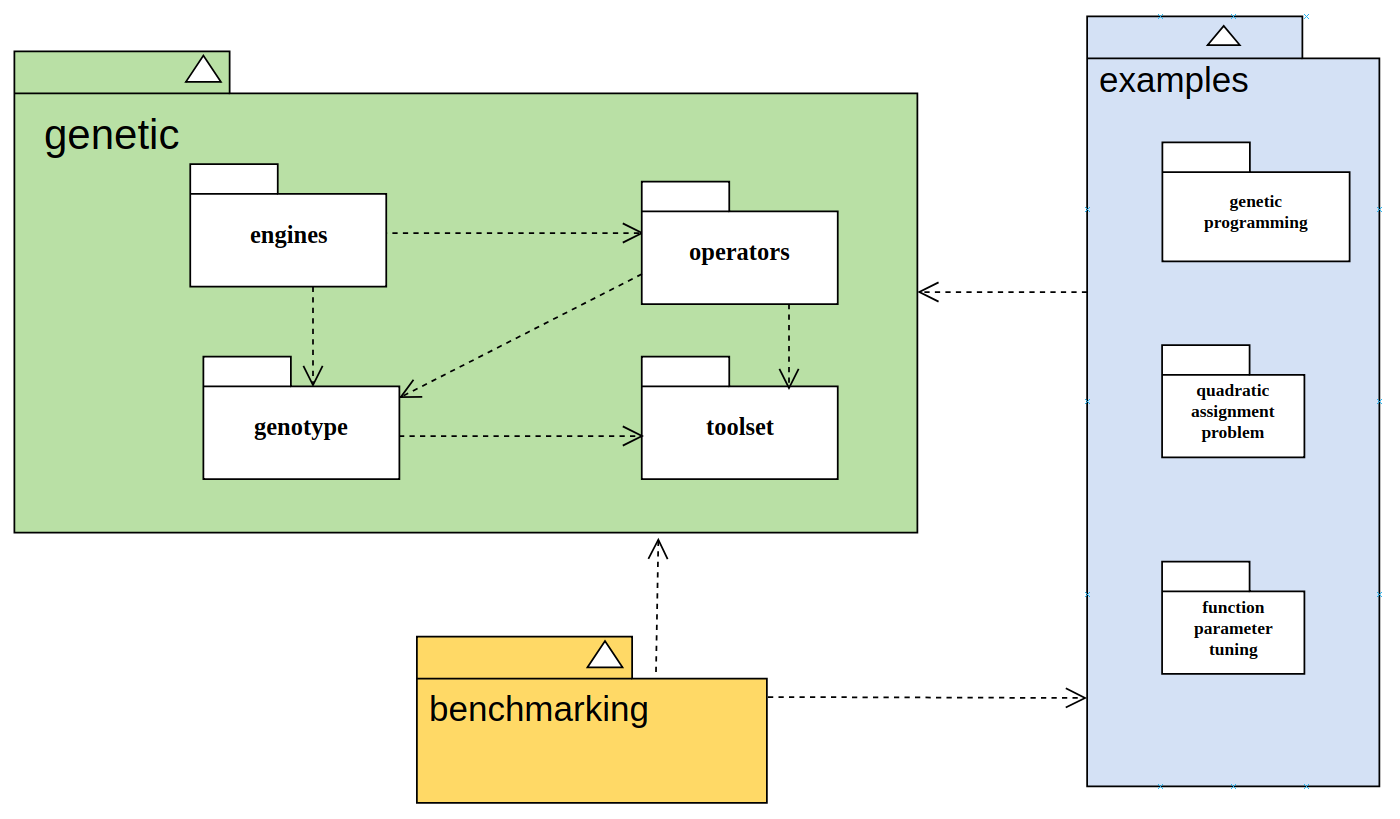
\includegraphics[width=1.\textwidth]{img/diagrams/alleles-top-packages}
\caption{Packages and their source dependencies}\label{diag:packages}
\end{figure}

\textit{genotype} package contains classes, which correspond to the information used to describe behavior of an individual. This is achieved using 4 type classes: \textit{Fitness, Join, Modification} and \textit{Scheme}. This subpackage also contains \textit{CachedFitness} class, which is a wrapper around provided fitness function, with additional caching behavior \ref{diag:genotype-classes}. 

\begin{figure}[h]
\centering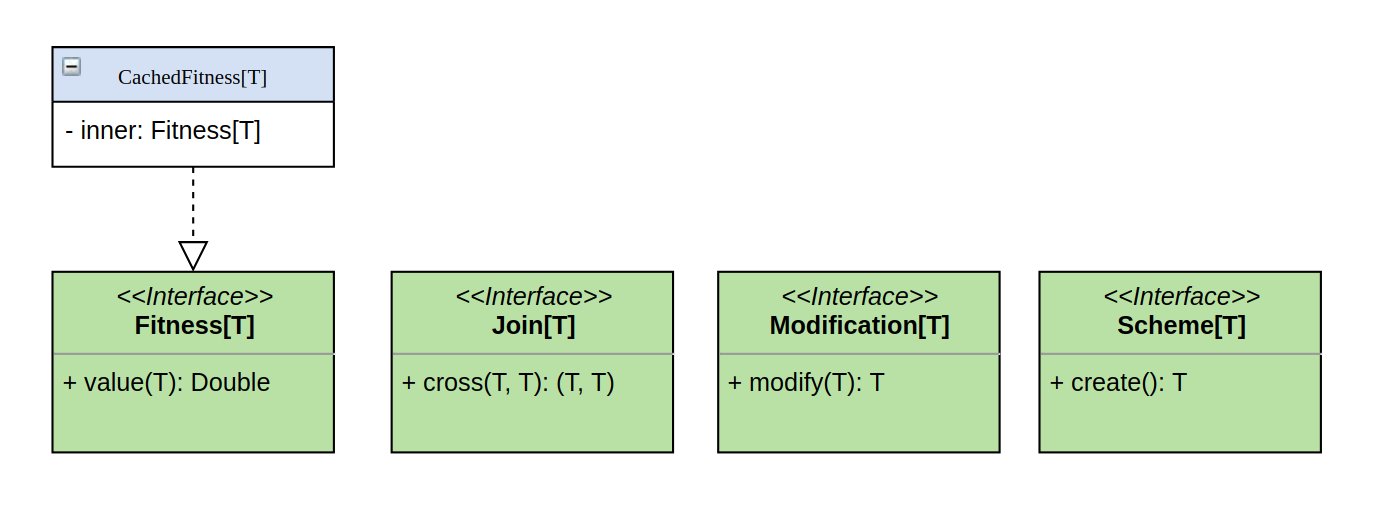
\includegraphics[width=1.\textwidth]{img/diagrams/alleles-genotype}
\caption{Type classes used to describe an individual}\label{diag:genotype-classes}
\end{figure}.

\textit{engines} package contains the heavy part of genetic algorithm implementation. Here one may find EvolutionEnvironment class and its concrete implementations. Every child class (parallel implementation) is placed in its specific subpage, so users have to import only the part, which they are interested in or everything, if this is desired. This approach may be seen in project structure \ref{diag:project-structure}, where the interfaces, which are communicating between each other are placed at the top of the package and different variants of their implementation are placed into specific subpackage, which later is important for user needs.

\smallskip\textit{This satisfies predefined non-functional requirement \ref{nfreq:modul}}

\begin{figure}
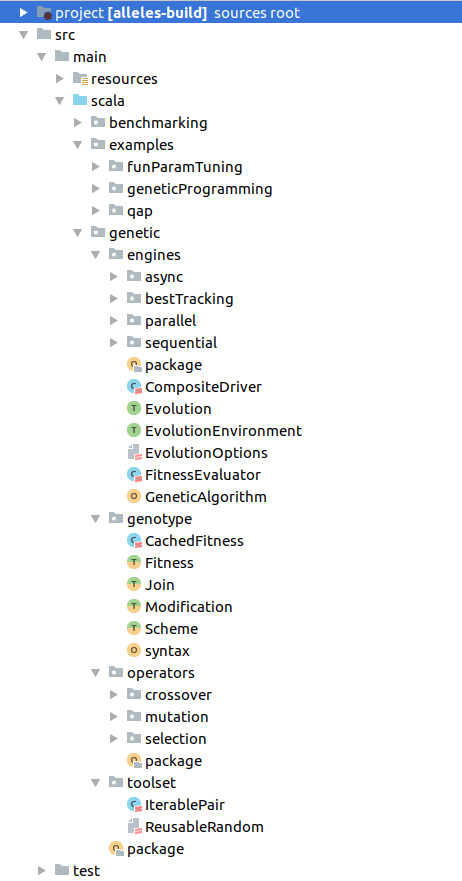
\includegraphics[width=.7\textwidth]{img/diagrams/alleles-project-structure}
\caption{Expanded project structure}\label{diag:project-structure}
\end{figure}

\medbreak
The way in which parts of \textit{engines} package are related to each other may be observed in \textit{genetic} class diagram\ref{diag:genetic-classes}

\begin{figure}
\centering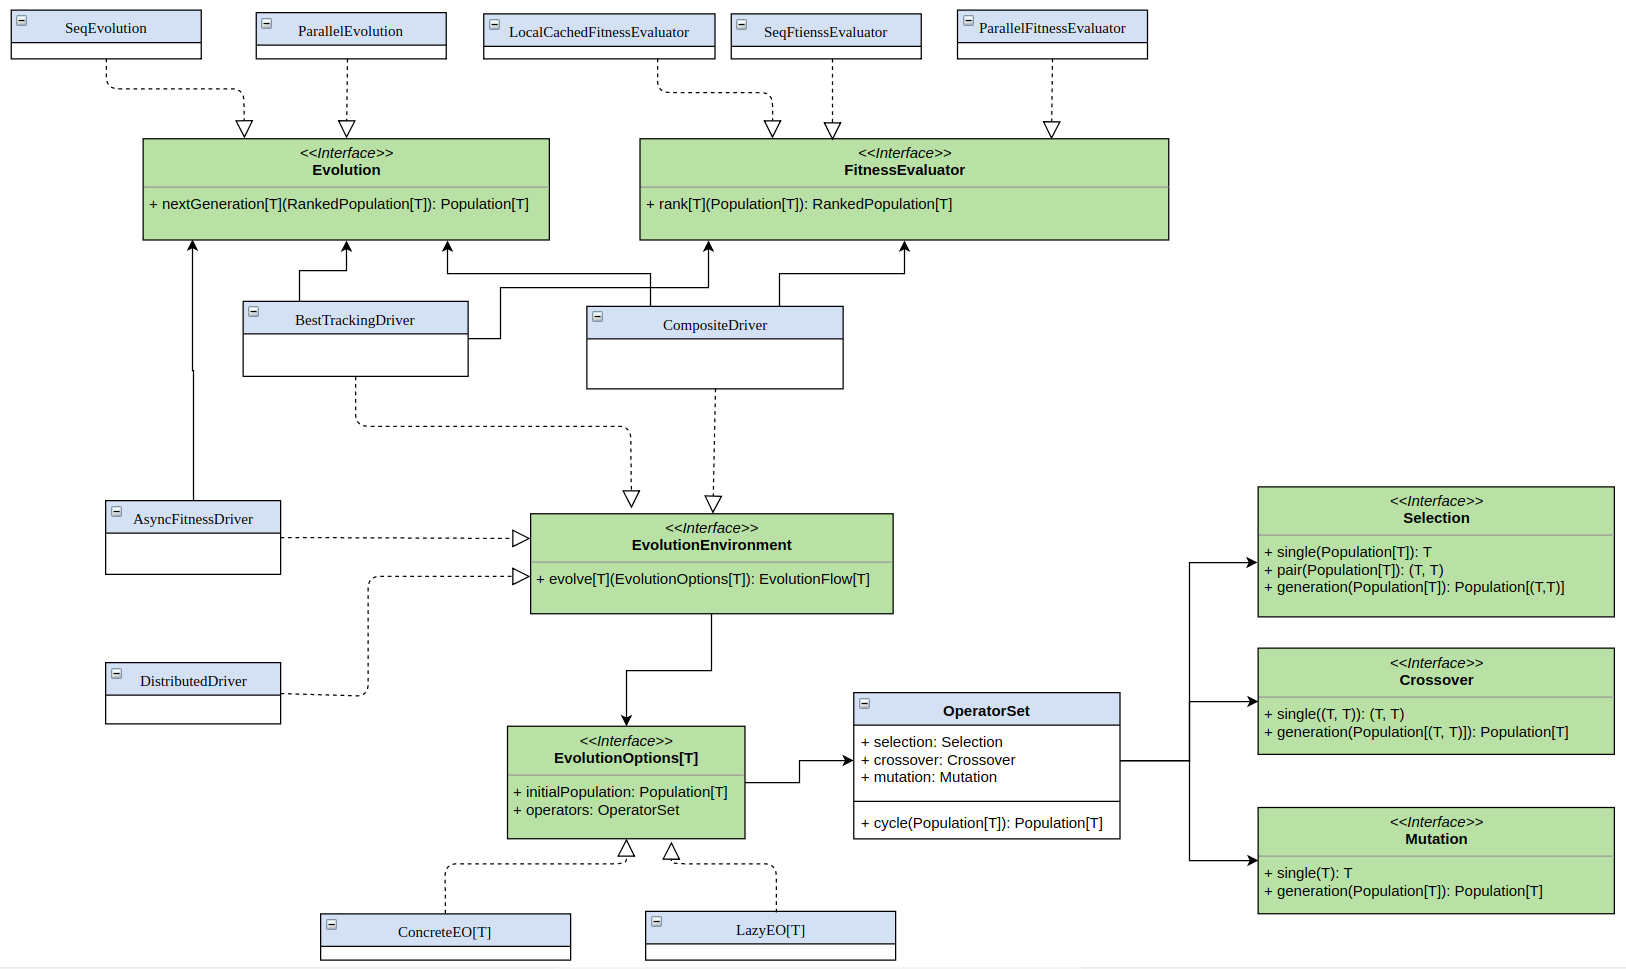
\includegraphics[width=1.\textwidth]{img/diagrams/alleles-genetic-class}
\caption{Classes diagram from \textit{genetic} package}\label{diag:genetic-classes}
\end{figure}

\section{Usage}
The library artifact may be added into the project as dependency using maven tool or sbt. After this, if library requirements are met, imported classes are ready to be used.

\subsection{Requirements}
\begin{itemize}
\item Scala 2.12.6
\item sbt 1.2.1
\item Apache Spark 2.3

\end{itemize}

\bigbreak
\subsection{API}
Here is described the application programming interface of the library. Due to its specific type, the frameworks do not usually have use case diagram defined, but instead present its value through API. It is brief description of the classes and functions available to a user, in which they communicate and actually use a programming library.\footnote{Description of the rest of the classes was ommited due to its large size}

\begin{itemize}

\item \texttt{trait EvolutionEnvironment}

	\begin{itemize}
		\item \texttt{def evolve[T: Fitness : Join : Modification](options: EvolutionOptions[T]): EvolutionFlow[Population[T]]}

		Creates an evolution flow out of evolotuion options of type T, with available implicit objects of class Fitness[T], Join[T], Modification[T]
	\end{itemize}

\smallskip
\item \texttt{type EvolutionFlow[T] = akka.util.Source[T, NotUsed]}

A type alias to akka-streams Source. Contains all the methods of akka.util.Source

\smallskip
\item \texttt{trait EvolutionOptions[T]}

A trait which holds the parameter for constructing evolution flow
\begin{itemize}
	\item \texttt{def initialPopulation: Population[T]}
	\item \texttt{def operators: OperatorSet[T]}
\end{itemize}

\smallskip
\item \texttt{trait Evolution}

Corresponds to the one step long evolution. Derives rated population to the new one using \texttt{class OperatorSet}
\begin{itemize}
	\item \texttt{def nextGeneration[T: Join : Modification](ratedPop: Population[Rated[T]], operators: OperatorSet): Population[T]}
\end{itemize}

\smallskip
\item \texttt{class FitnessEvaluator}

A class which basing on the instance of Functor[Population[T]] computes the fitness values for the population.
\begin{itemize}
	\item \texttt{def rate(population: Population[T]): Population[Rated[T]]}
\end{itemize}

\smallskip
\item \texttt{trait Fitness[T]}
\begin{itemize}
	\item \texttt{def value(t: T): Double}
	
	Computes the fitness value for an individual of type \texttt{T}

	\item \texttt{def cached: CachedFitness[G]}

	Returns a cached version of this fitness function
\end{itemize}

\smallskip
\item \texttt{trait Join[T]}
\begin{itemize}
	\item \texttt{def cross(a: T, b: T): IterablePair[T]}

	Mixes a pair of individuals into new pair with shared genome
\end{itemize}

\smallskip
\item \texttt{trait Modification[T]}
\begin{itemize}
	\item \texttt{def modify(t: T): T}

	Returns modified version of parameter \texttt{t}
\end{itemize}

\smallskip
\item \texttt{trait Scheme[+T]}
\begin{itemize}
	\item \texttt{def create: T}

	Creates a new instance of type \texttt{T}
\end{itemize}

\smallskip
\item \texttt{trait Selection}
\begin{itemize}
	\item \texttt{def single[T](population: Population[Rated[T]]): (T, T)}

	Selects a single pair from the Population of rated individuals 

	\item \texttt{def generation[T](population: Population[Rated[T]]): Population[(T, T)]}

	Selects pairs of individuals into new population of the same size
\end{itemize}

\smallskip
\item \texttt{trait Crossover}
\begin{itemize}
	\item \texttt{def single[T: Join](parents: (T, T)): IterablePair[T]}

	Mixes one pair of individuals with provided \texttt{Join[T]} instance 

	\item \texttt{def generation[G: Join](population: Population[(G, G)]): Population[G]}

	Mixes every pair of given population into the new population with provided \texttt{Join[T]} instance
\end{itemize}

\smallskip
\item \texttt{trait Mutation}
\begin{itemize}
	\item \texttt{def single[T: Modification](individual: T): T}

	Mutates a single individual with the \texttt{Modification[T]} instance 

	\item \texttt{def generation[T: Modification](population: Population[T]): Population[T]}

	Mutates all population with the \texttt{Modification[T]} instance
\end{itemize}

\end{itemize}

% Table 1. Spark framework RDD usage.

%\subsection{Preimplemented algorithms}
%\textit{ToDo - add info}

%\subsection{Evolution interruption}
%\textit{ToDo - add info}

\section{Meeting the predefined requirements}

With current implementation all predefined functional and non-functinal requirements were successfully met.

\chapter{Experiments}

The purpose of experiments is to observe common patterns, that allow a better understanding of the system, which may be used for optimization, customization and improvement needs. In this chapter will be studied the benefits, which may be achieved be applying parallelization to any of the used algorithms.

\section{Testing environment}

In order to run experiments objectively and make fair conclusions, it is important to set the testing environment, which is going to be the same for every test run.

\subsection{Settings}

The experiments will be performed on one of the implemented examples of library usage. This is the solution for the Quadratic Assignment Problem. It is one of the fundamental combinatorial optimization problems in the branch of optimization or operations research in mathematics, from the category of the facilities location problems. For this purposes could have been used any problem, as in order to make conclusions, the results will be compared with each other.

Here is a list of the parameters mutual to every test:
\begin{itemize}

\item Optimization problem

The experiments will be performed on one of the implemented examples of library usage -  Quadratic Assignment Problem. It is one of the fundamental combinatorial optimization problems in the branch of optimization or operations research in mathematics, from the category of the facilities location problems. For this purposes could have been used any problem, as in order to make conclusions, the results will be compared with each other.


\item Genetic operators

For the evolution flow, the set operators stay unchanged. It contains tournament selection strategy with the size of 20, one point crossover and simple chromosome swap mutation. These parameters have been left immutable in order to minimize parameter noise during experiments.

\end{itemize}

Other algorithm parameters like the number of iterations, size of the population and complexity of fitness function will be regularized in order to examine the correlation.

\subsection{Hardware}

The experiments were performed using two machines with a different configuration, motivated by the different results, which may be observed depending on the used machine.

\begin{table}[h]
\centering\caption{Hardware characteristics \label{tab:exp-hardware}}
\begin{tabular}{|l|c|c|c|}
\hline
\textbf{Label} & \textbf{Operating system} & \textbf{Total RAM} & \textbf{vCPU cores} \\
\hline
Machine \#1 & Windows 10 & 16 GB & 8 \\
\hline
Machine \#2 & Ubuntu 18.04 & 8 GB & 4 \\
\hline
\end{tabular}
\end{table}

\section{Sequential behavior}

In order to be able to make some conclusions having the data from experiment runs, it is important to know how the system behaves in sequential runs. This configuration may also be considered as one with parallelism level 1.

Run parameters:
\begin{table}[h]
\centering\caption{Hardware characteristics \label{tab:exp-hardware}}
\begin{tabular}{|l|c|c|c|}
\hline
\textbf{Parameter} & \textbf{Value}  \\
\hline
Number of iterations & 10 \\
\hline
Size of population & 5000 \\
\hline
Fitness function duration & ~5 ms \\
\hline
\end{tabular}
\end{table}

After the run with a sequential implementation of GA here is a plot of processor resources usage over time \ref{img:cpu-run-1}. It is clear that only one virtual CPU core is working on its full speed at a time, but there is no virtual CPU core, which runs all the evolution, as after some time it is changed to another core. In the meanwhile, there bumps on other cores every some time. This is garbage collector sessions, as by default JVM runs GC on the free cores in order to minimize actual working time.

\begin{figure}[h]
\centering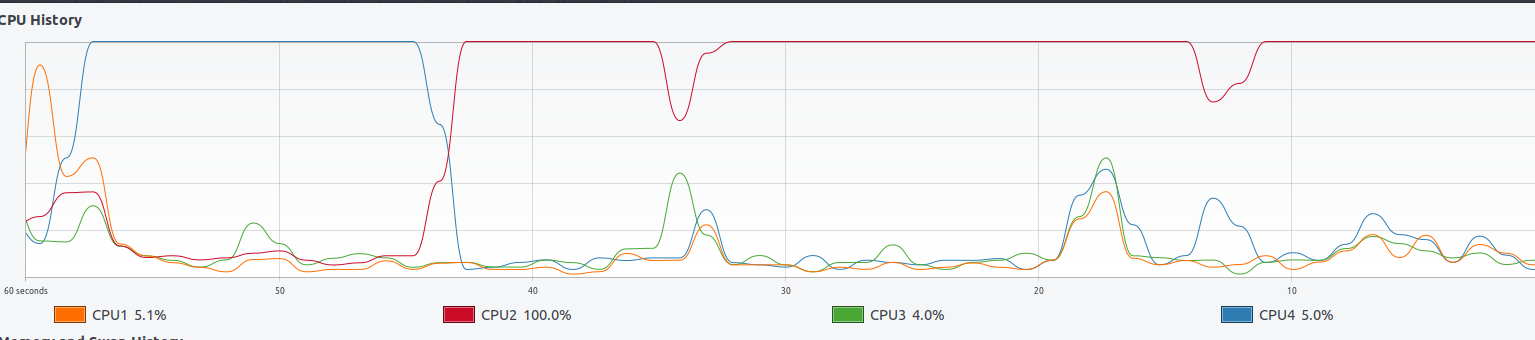
\includegraphics[width=1\textwidth]{img/exp/1/cpu-500}
\caption{CPU load during test run \#1}  \label{img:cpu-run-1}
\end{figure}

To test whether conjecture about GC runs is actually true for the next run the size of a population was increased to 50000 and fitness function time reduced to 0.5 ms. This should increase the number of objects allocated during a given time segment, resulting in more frequent garbage collector sessions. Here are the observations over CPU status during the run \#2 \ref{img:cpu-run-2}. This plot confirms the previous assumption - number of load rises is much bigger, as a lot more object are allocated and deallocated. Nevertheless, CPU usage in example \#2 in some aspects is similar to the CPU usage during run \#1: there is only one virtual CPU working for 100\% at a time and the rest of virtual cores are working on additional job, such as garbage collection or scheduling.

\begin{figure}[h]
\centering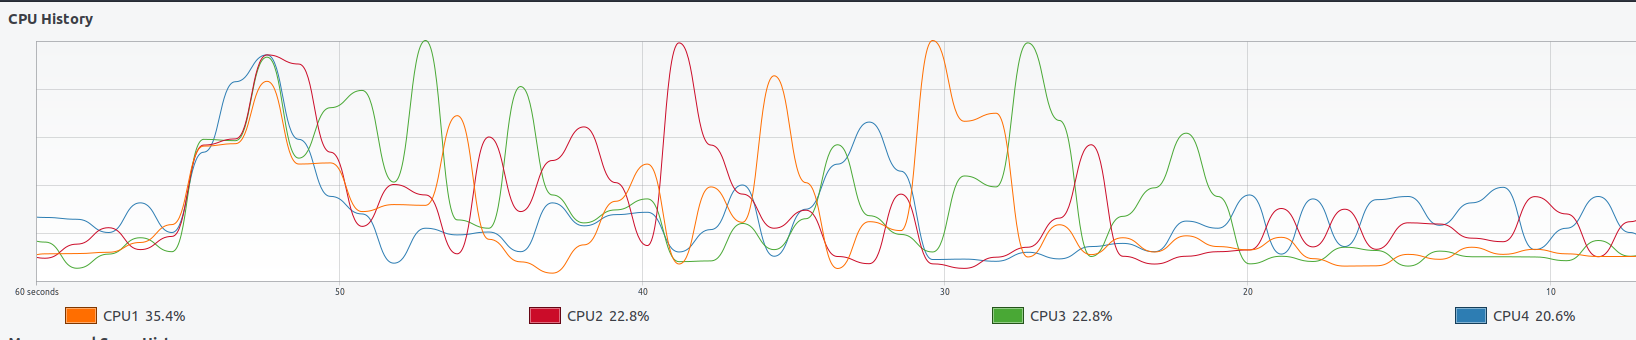
\includegraphics[width=1\textwidth]{img/exp/1/cpu-5000}
\caption{CPU load during test run \#2}  \label{img:cpu-run-2}
\end{figure}

The important conclusion from these runs is that even during sequential computations JVM still uses other available cores to optimize working time. For this reason, when using more than one CPU core for the purpose of an algorithm, JVM may find no free cores and will schedule garbage collection together with other computations, which will naturally result in a downturn of performance. \textbf{This is one of the reasons, why the speed-up from parallelization is not ideally linear to the number of added cores.}


\section{Measuring parallelization impact}

In this section will be measured performance increase in different thread pool configuration.
Performance of each configuration will be measured and compared to the performance of sequential run without thread pool limitation. The goal of the experiment is to find how much of the performance may be gained by using parallelization with limited number of execution cores and  what kind of configuration provides the best performance characteristics of the algorithm.

\subsection{Performance increase}

By applying a thread pool, depending on its type, an application is restricted to use no more or exact number of threads to its purposes. This also includes garbage collection, so the statement that sequential run is equal to parallel with limited pool to one thread is not true, as in the former case garbage collection may be scheduled on the other thread by JVM, wherein the letter - one thread is responsible for all actions. This is why parallelization with a small number of threads gives a very small speed-up.

The measurements can be found in tables \ref{tab:comp-ubuntu} and \ref{tab:comp-windows} in comparison to sequential run values placed in \ref{tab:win-ub-perf}.

\begin{table}[h]
\centering\caption{Performance of sequential configuration of genetic algorithm \label{tab:win-ub-perf}}
\begin{tabular}{|c|c|c|c|}
\hline
\textbf{Machine} & \textbf{Taken time} & \textbf{Population size} \\
\hline
Machine \#1 & 1725 ms & 10000 \\
\hline
Machine \#2 & 1779 ms & 10000 \\
\hline
\end{tabular}
\end{table}

\begin{table}[H]
\centering\caption{Performance speedup depending on available threads comparing with sequential run on machine \#1 \label{tab:comp-windows}}
\begin{tabular}{|c|c|c|c|}
\hline
\textbf{Number of threads in the pool} & \textbf{Taken time} & \textbf{Performance increase} & Available vCPU cores \\
\hline
2 & 1276 ms & 35.2\% & 8 \\
\hline
4 & 509 ms & 238\% & 8  \\
\hline
8 & 345 ms & 400\% & 8 \\
\hline
16 & 328 ms & 426\% & 8 \\
\hline
32 & 296 ms & 482.7\% & 8 \\
\hline
64 & 300 ms & 475\% & 8 \\
\hline
100 & 305 ms & 465.6\% & 8 \\
\hline
\end{tabular}
\end{table}

\begin{table}[h]
\centering\caption{Performance speedup depending on available threads comparing with sequential run on machine \#2 \label{tab:comp-ubuntu}}
\begin{tabular}{|c|c|c|c|}
\hline
\textbf{Number of threads in the pool} & \textbf{Taken time} & \textbf{Performance increase} & Available vCPU cores \\
\hline
 2 & 1247 ms & 42.6\% & 4 \\
\hline
 4 & 640 ms & 177\% & 4 \\
\hline
 8 & 564 ms & 215\% & 4 \\
\hline
 16 & 576 ms & 208\% & 4 \\
\hline
 32 & 592 ms & 200.5\% & 4 \\
\hline
\end{tabular}
\end{table}

Using graph visualizations \ref{img:ub-perf}, \ref{img:win-perf} it is shown, that slope of performance increase is independent from machine or operating system. 

\begin{figure}[H]
\centering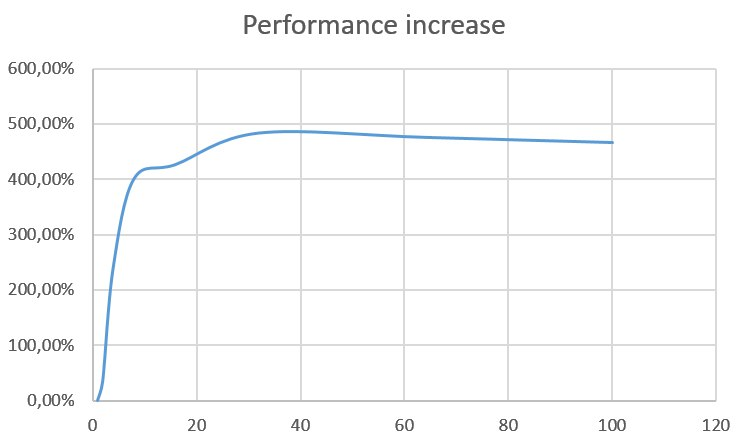
\includegraphics[width=.8\textwidth]{img/exp/2/windows-performance-increase}
\caption{Visualization of performance increase per available threads on machine \#1}  \label{img:win-perf}
\end{figure}

\begin{figure}[h]
\centering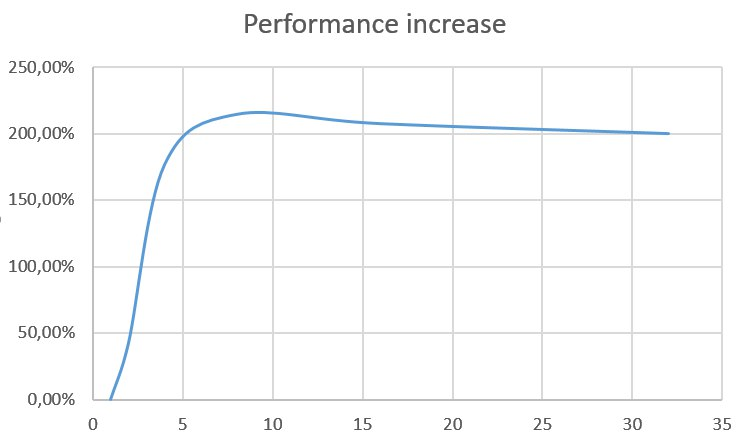
\includegraphics[width=.8\textwidth]{img/exp/2/ubuntu-performance-increase}
\caption{Visualization of performance increase per available threads on machine \#2}  \label{img:ub-perf}
\end{figure}

From observations it also appears, that \textbf{optimal point of performance gain is approximate to \( 2 * n\) threads available in case of the fixed thread pool, where \(n\) is number of virtual CPU cores available on the machine.}

\subsection{CPU Load}

While testing how different thread pools applied to an application changing its overall performance, it is also important how the hardware is supporting this growth. So in order to a better understanding of the nature of performance, the machine CPU load was measured.
For this matter the algorithm configuration was changed, so it is possible to observe the patterns on CPU usage plots: size of a population increased to 100000 and the number of iterations increased to 30. 

Here may be found screenshots from the resource monitoring tool, taken while running the application with different configurations \ref{img:cpu-thread-2}, \ref{img:cpu-thread-4}, \ref{img:cpu-thread-8}, \ref{img:cpu-thread-16}, \ref{img:cpu-thread-32} (all runs were performed on machine \#2 with 4 virtual CPU cores).

\begin{figure}[h]
\centering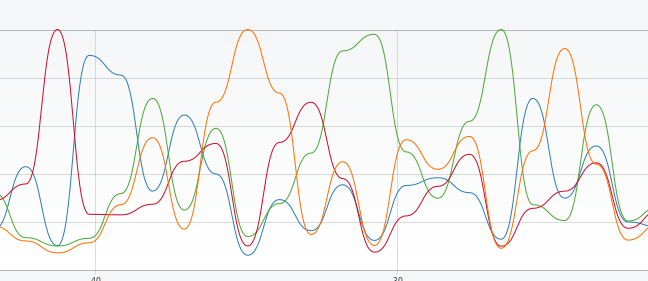
\includegraphics[width=0.95\textwidth]{img/exp/2/limit-threadpool-2}
\caption{The CPU load while processing GA evolution limited by a thread pool with fixed size 2 }  \label{img:cpu-thread-2}
\end{figure}

\begin{figure}[H]
\centering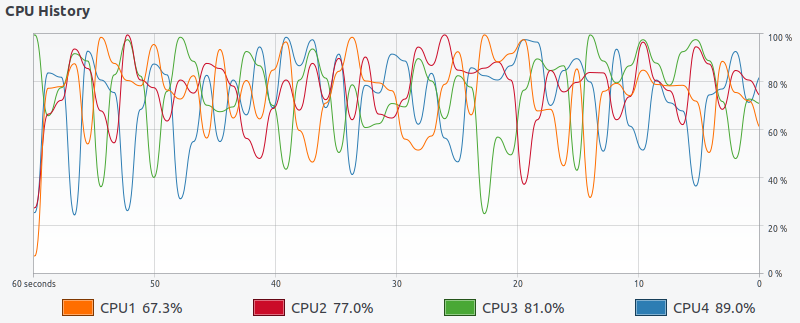
\includegraphics[width=0.95\textwidth]{img/exp/2/limit-threadpool-4}
\caption{The CPU load while processing GA evolution limited by a thread pool with fixed size 4 }  \label{img:cpu-thread-4}
\end{figure}

\begin{figure}[H]
\centering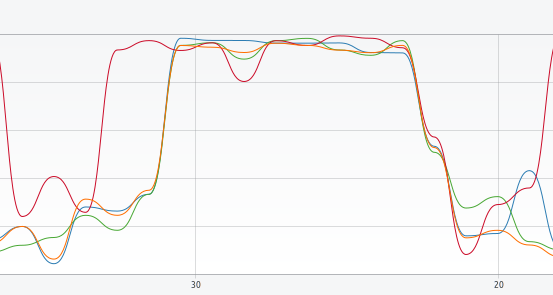
\includegraphics[width=0.95\textwidth]{img/exp/2/limit-threadpool-8}
\caption{The CPU load while processing GA evolution limited by a thread pool with fixed size 8 }  \label{img:cpu-thread-8}
\end{figure}

\begin{figure}[H]
\centering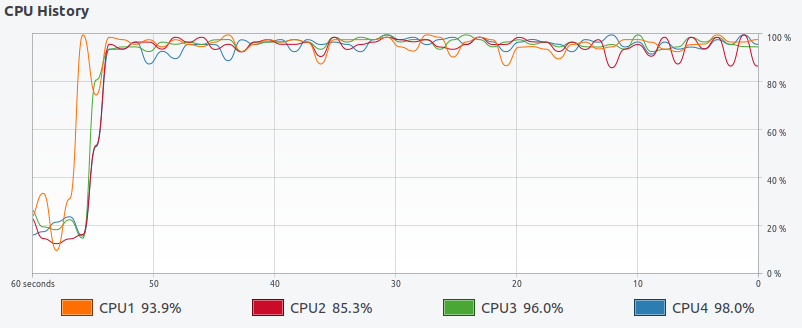
\includegraphics[width=0.95\textwidth]{img/exp/2/limit-threadpool-16}
\caption{The CPU load while processing GA evolution limited by a thread pool with fixed size 16 }  \label{img:cpu-thread-16}
\end{figure}

\begin{figure}[H]
\centering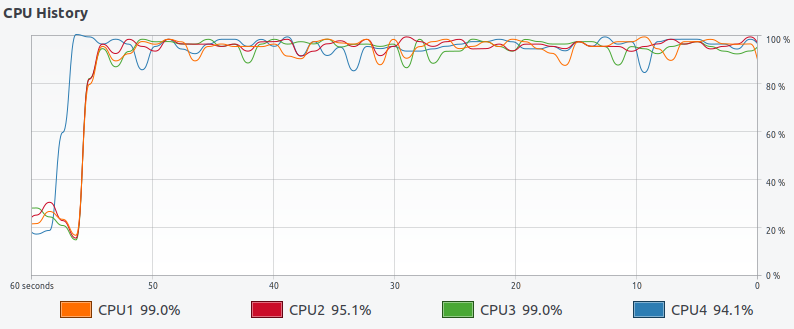
\includegraphics[width=0.95\textwidth]{img/exp/2/limit-threadpool-32}
\caption{The CPU load while processing GA evolution limited by a thread pool with fixed size 32 }  \label{img:cpu-thread-32}
\end{figure}

These plots correspond to the virtual CPU cores workloads during the algorithm run. In order to achieve the highest performance, the maximum amount of work should be done in a time segment, so the CPU load should be the highest. When applying a  thread pool with 2 available threads, having 4 virtual CPU cores, task scheduler is jumping from one core to another, keeping average CPU load near 60\%. This confirms low-performance increase, comparing to bigger thread pools. Later with each next thread pool configuration applied the average CPU load increases with the number of available threads, reaching its peak with 16-thread pool on 95\% (some of the resources are reserved for the operating system, preventing running processes - JVM in this case - from corrupting machine state). When running the application on 32 threads, which is 8 times more than available virtual CPU cores, average CPU load is nearly the same, with more resources assigned to keep the thread scheduling, which together corresponds to the smaller performance gain, compared to a 16-thread pool. On this level parallelization job scheduling and switching between different tasks are taking more resources, which could have been used for ``business'' computations. \textbf{Basing on the observations, running the application with minimum I/O manipulations, it is optimal to keep the number of threads per virtual CPU core near 2-3, which directly correlates with performance increase discussed in the previous section}.


\chapter*{Conclusions}

Nowadays there is extra attention gathered near artificial intelligence breakthroughs. It has already started to change the lives of people, who are not relative to any of computer science domains. Nevertheless, behind a spectacular achievements hides a lot of hard work of many people, trying to push existing boundaries forward. This condition is absolutely necessary for the progress to keep going. New algorithms and techniques are integrated with the existing domains every year, however some of the methods, which make these results possible were already developed many years ago, waiting for their time to come (a great example may serve a history of neural networks). It is important to embrace existing solutions in order to make them better, fix their flaws.

The thesis introduces a new way of developing and integrating genetic algorithm into existing applications and optimizing them using local parallelization and distributed computing. It serves users as a toolkit containing predefined solutions, which are open for users in terms of choosing and combining them together into consistent algorithm. Using state of the art technologies and advanced programming techniques, it was possible to implement a solution for addressed flaws of genetic algorithms. In order to gain user base the future enhancements should be aim to simplify the process of developing GA for the end user, by enabling them to use more predefined strategies of selection, crossover and mutation ready for user. It also necessary for the library to be developed and discussed in open-source community. Future work should be done to popularize this solution and present it to the wider community of academia world, as well as day-to-day developers.

\iffalse

\chapter*{Zakończenie}

W pracy udało mi się dużo zrobić. \lipsum[17]

Mnóstwo innych rzeczy da się poprawić i rozwinąć. \lipsum[23]



\appendixpage
\appendix
%\addappheadtotoc

\chapter{To powinien być dodatek}\label{Dod1}

\lipsum[9-11]

% W pracy pojawią się tylko prace naprawdę cytowane.
% \nocite{*}

\fi

\bibliography{literatura}
\bibliographystyle{dyplom}

\end{document}
